Humans are visual in nature and as such we have constructed our world
around visual cues. We use written street signs rather than, say,
smells or sounds to navigate the road network because our biological
vision system has both higher fidelity and wider bandwidth than other
senses. In order for computers to understand and interact with our
world we must either develop automated vision systems or re--signpost
our world. Computer vision is the endeavour to take the former route.

This thesis addresses the problem of developing a computer vision
system that understands the geometry of the environment at a
semantically meaningful level. By ``semantically meaningful'' we mean
at the level of objects and events relevant to humans and human
interactions, as in the difference between an city roadmap (which we
would say is semantically meaningful on account of its high--level
representation of quantities such as roads and addresses) and a set of
3D points in space. Our goal is to recover semantically meaningful models
of the world from visual input.

To this end we explore two types of models. The first relates
low--level photometric information directly to high--level concepts
such as the function of an environment and the location of objects
within it. Building on recent progress in contextual computer vision,
we show how to derive visual context directly from an environment's
texture structure. The second type of model we explore relates images
to high--level concepts via an intermediate representation of
high--level scene geometry. Contrary to much previous work in
geometric computer vision, we select a representation that leads
naturally to semantic--level reasoning tasks such as place recognition
and object detection, for which we argue that the indoor Manhattan
model is an attractive choice. Much of this thesis concerns the
estimation of indoor Manhattan models from single and multiple images.

\section{Motivation}

The research presented here has been motivated from a variety of
angles over time. This thesis was originally motivated by the
application area of augmented reality (AR). In the broadest sense, AR
systems aim to overlay relevant information onto a human's visual
field--of--view. One important challenge is to build a 3D model of the
environment and track the sensor with respect to it in order to create
the illusion of annotations that move with 3D objects in the
environment. This problem is known as simultaneous localisation and
mapping (SLAM), and has seen great progress over the past several
decades. In particular, visual SLAM, in which the sensing apparatus is
a camera, has taken great strides, moving from single rooms to a
entire cities, and from costly off--line processing to real--time
systems. However, in order to select relevant information and have
annotations interact seamlessly with other visual stimulus, the AR
system must have some understanding of the visual world beyond the
low--level point clouds generated by SLAM systems.

It is neither surprising nor objectionable that so much effort towards
AR has focused on visual SLAM, but now that high--performance SLAM
systems \textit{are} available, the question that naturally presents
itself is: \textit{are we done yet?} In this thesis we will argue that
while SLAM is an important first step, many challenging and general
computer vision problems remain to solve before AR systems can be
fully realised. For example, the relevance of certain types of
information to the wearer varies with the type of environment that the
wearer is moving within. Directions to a restaurant may be relevant
while outdoors but directions to the kitchen are less likely to be
helpful within the wearer's own house. Within the home, the
augmentations most useful in the kitchen are likely to be different to
those suitable to the bedroom. Furthermore, the likely locations of
various objects is tightly coupled to the surfaces and boundaries
within an environment. A human would not search for lost keys on the
ceiling first, nor outside a window, but to make this inference an AR
system must first identify key surfaces and their orientations. These
problems are not immediately solved by the ability to locate oneself
within an arbitrary 3D coordinate frame, though a major theme of this
thesis is how to use such information together with other image
evidence for high--level reasoning tasks.

Although this thesis was originally motivated by applications within
AR, much inspiration was drawn from the single--view computer vision
literature, principally from the literature dedicated to \textit{scene
  understanding}, which is the problem of understanding images in
terms of objects, actions, and semantically meaningful geometric
primitives. Scene understanding has a long history within the
single--view computer vision literature but a shorter history within
the multiple--view literature. One motivation for this
research is the extension of traditional scene understanding
techniques to the context of multiple views. This is a challenging
problem because single--view techniques are commonly cast in terms of
rectangular arrays of pixels, which do not naturally incorporate the
kind of geometric information available in a multiple view context.

There is a very large literature on single--view scene understanding, and a
corresponding plethora of models to choose from. The focus of this
thesis is on the extraction of high--level geometric information
within indoor--type environments, with relevance to scene
categorisation and object localisation. The hope is that this problem
is large enough to be interesting, small enough to be tractable, and
perhaps insightful enough to be instructive for future research in
the relatively new domain of multiple--view scene understanding.

There are many reasons that utilising multiple views is an attractive
direction for scene understanding research. Firstly, video on the
internet has become increasingly important over the past several
years, increasing the relevance of computer vision systems that
process video streams rather than single images. Secondly, mobile
phones have become more attractive devices for vision systems as the
processors and cameras now ubiquitously attached to them continue to
become more powerful. Finally, depth sensing cameras have entered the
mainstream consumer hardware market and are likely to become more
common over the coming years.

\section{Our Approach}

\begin{figure}[tb]%
  \centering
    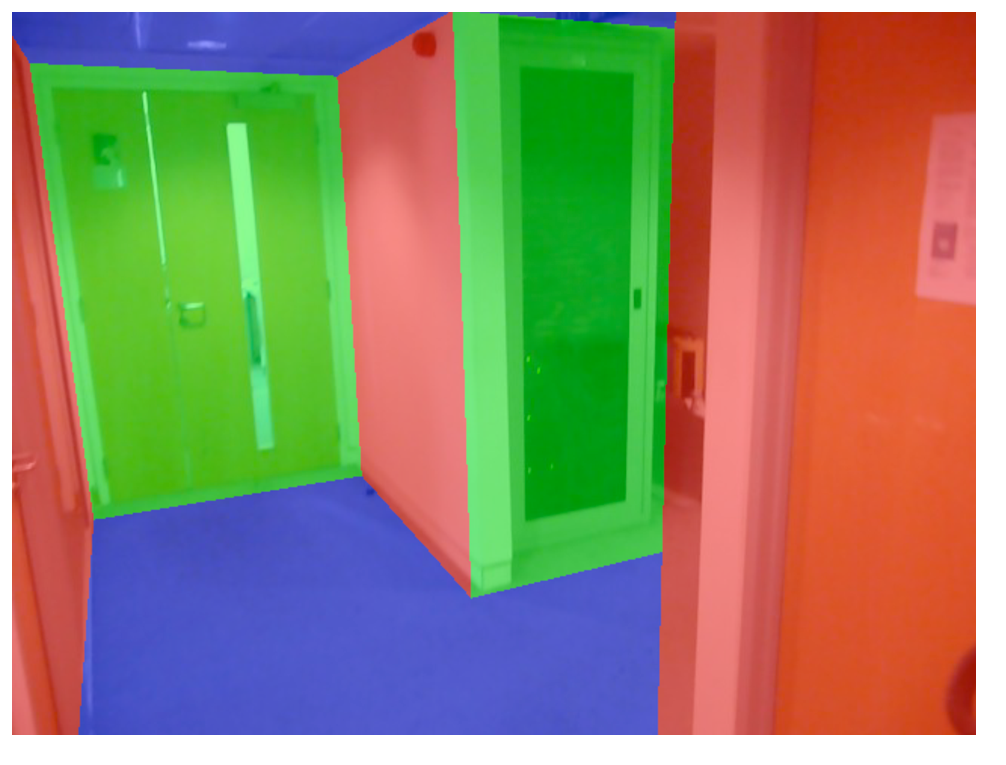
\includegraphics[width=0.5\textwidth]{manhattan-scene}
    \caption{An example of an indoor Manhattan scene.}
  \label{fig:manhattan-eg}
\end{figure}

In this thesis we present two approaches to deriving semantic--level
scene information from visual input. 

\subsection{Photometric Models}

The first model we present is a purely photometric approach and builds
on ideas from texture analysis, in particular the texton model. This
model associates each pixel with a discrete texture element, which is
then related to the semantic--level variable of interest. We show how
textons can be leveraged toward the problems of scene recognition and
contextual object search. Despite the simplicity of this approach, we
show that it is effective for the proposed problems.

In contrast to systems based on edges, interest points, or local
descriptors, utilising texture information allows us to leverage
visual information in non--salient image regions. This is particularly
important for environments in which there are few individually
distinctive image patches, yet the overall scene appearance conveys
significant information.

We present qualitative results motivating the use of texture structure
for the stated task, followed by a formal probabilistic model and
quantitative comparisons with the state--of--the--art.

\subsection{Coarse Geometric Models}

The second part of this thesis focuses on capturing geometric
information in a form well--suited to semantic--level reasoning. This
represents a departure from much of the scene understanding
literature, in which geometric information is captured implicitly,
rather than via explicit geometric assumptions. Our decision to work
with explicit geometric models is motivated by the observation that
much about scenes and objects is tied to the high--level shape of the
environment, particularly the location of major surfaces and
boundaries.

As a simple illustration of this, consider the image shown in
\figref{manhattan-eg}. Despite the low information content of the
image -- it is defined by just a handful of vertices -- a human can
make many high--level inferences about this environment, including
answers to questions such as (in order of increasing difficulty):
\begin{enumerate}
  \item{What is the direction of gravity?}
  \item{Where would doors most likely be found?}
  \item{Where would a person be most likely to stand and at what scale?}
  \item{Is this an office or a house?}
  \item{What is the absolute scale of the environment?}
\end{enumerate}

While the image does not provide enough information for definitive
answers to any of these questions, it does provide surprisingly strong
evidence given that it consists of just a few hundred bits of
information. Thus it seems that coarse geometric information is
particularly valuable for high--level inference.

The image in \figref{manhattan-eg} shows one example of an indoor
Manhattan environment \cite{Lee09}, which is the hypothesis class we
adopt for geometric reasoning in this thesis. Under this model the
world is composed of a floor plane, ceiling plane, and a set of
vertical walls that meet at vertical edges. Indoor manhattan
environments constitute a subset of the more general set of Manhattan
environments, in which any arrangement of surfaces in three dominant
directions is permitted. It is an attractive model for a number of
reasons. Firstly, as argued above, it captures geometric information
of high value for semantic--level reasoning. Secondly, despite the
strong geometric assumptions, a surprisingly broad range of
environments can be represented exactly or approximately as indoor
Manhattan models. Thirdly, strong geometric assumptions assist in the
interpretation of ambiguous image evidence, since salient information
in one region can constrain the interpretation of other
regions. Finally, an efficient inference algorithm exists for this
hypothesis class, which is the subject of later chapters.

There is no hard distinction between a ``geometry--less'' and a
``geometry--laden'' approach to scene understanding. In either case
one is drawing probabilistic inferences from images; the distinction
is in how those inputs are combined, which conditional independences
are assumed, and how the hypothesis class is formulated. Our choice to
incorporate geometry corresponds to a particular choice of
independence assumptions, which differ from those typically chosen in
photometrically inspired models. This thesis is concerned with the
recovery of geometry for the sake of the high--level inference that it
enables, not for the sake of the geometry itself, and our choice of
model reflects this.

\section{Exegesis}

The remainder of this thesis is organised as follows. Chapter 2
presents a review of literature relevant to this thesis. Due to the
connection of our work to the traditionally disparate fields of SLAM
and scene understanding, the literature review breaks down into scene
understanding work that has touched on geometry, and SLAM work that
has touched on scene understanding.

Chapter 3 presents an appearance--only approach to scene understanding
in the context of a moving camera. We work with textons as the basic
observation unit and present a probabilistic model connecting these to
scene categories and object locations.

We then begin the presentation of our work concerning indoor Manhattan
models. Chapter 4 presents the model formally, and covers various
geometric observations on which later chapters rest. There is little
prior work on the indoor Manhattan model, so we dedicate a full
chapter to defining the model formally and describing several useful
representations. We then turn in Chapter 5 to identifying the
orientation of three cardinal Manhattan directions given multiple
calibrated views. We show that estimating scene rotation jointly from
all available views is a dramatic improvement over the standard
approach of identifying vanishing points separately in each image. We
also show an order of magnitude improvement over approaches that use
surface normals estimated from a reconstructed point cloud.

Chapter 6 presents a probabilistic model relating sensor data to the
geometric quantities we wish to extract. We give separate
probabilistic models for photometric features, stereo data, and point
clouds, then we show how to combine these into a fully Bayesian model,
allowing our system to be easily tailored to a variety of contexts. We
present a dynamic programming algorithm that solves both
maximum--aposteriori and maximum--likelihood inference within our
model. This inference procedure is both fast and exact, making a
compelling alternative to previous approaches that explode
combinatorially in model complexity.

Chapter 7 presents a learning routine in which we learn to reconstruct
Manhattan environments based on training examples. We cast the
learning problem in a discriminative framework and use
state--of--the--art tools from the structured prediction
literature. We show that learning with respect to single versus
multiple views differs only by a change in feature space, and we
present extensive results for both contexts. 

Finally, chapter 8 summarises key results and suggests directions
for future work.
